\chapter{Аналитическая часть}

В данной части будет проведён анализ поставленной задачи, объектов трёхмерной сцены, а также существующих методов построения 3-х мерных сцен.

\section{Задача n тел}
\subsection*{Постановка задачи}
Пусть существует N частиц, представляемых материальными точками с массами $m_1, ..., m_N$, радиус векторами $\vec{r_1}, ..., \vec{r_N}$ и векторами скоростей $\vec{v_1}, ..., \vec{v_N}$ в момент времени $t=0$.
Попарное взаимодействие точек подчинено закону тяготения ньютона~\ref{eq:F_jk}.
\begin{equation}
	\label{eq:F_jk}
	\vec{F}_{jk} = G\hat{\vec{r_{jk}}}\frac{m_km_j}{\vec{r_{jk}}^2},
\end{equation}
где
\begin{itemize}
	\item $\vec{F}_{jk}$ -- Сила тяготения, действующая j-ой частицей на k-ю;
	\item $G = 6.67430 * 10^{-11} m^3s^{-2}kg^{-1}$ -- гравитационная постоянная, константа;
	\item $\vec{r_{jk}} = \vec{r_j} - \vec{r_k}$ -- вектор из точки k-ой частицы в точку j-ой;
	\item $\hat{\vec{r_{jk}}}$ -- единичный вектор из точки k-ой частицы в точку j-ой, задающий направление силы;
	\item $m_k, m_j$ -- массы k-ой и j-oй частиц соответственно.
\end{itemize}

Так как на k-ю частицу действую все остальные частицы системы с силами~\ref{eq:F_jk}, а также с учётом того факта, что силы аддитивны, получается сила, с которой все частицы системы действую на k-ю~\ref{eq:F_sumk}. 

\begin{equation}
	\label{eq:F_sumk}
	\vec{F}_{k} = Gm_k\sum_{j=1, j \neq k}^{N}{\frac{m_j}{\vec{r_{jk}}^2}\hat{\vec{r_{jk}}}}.
\end{equation}

Второй закон Ньютона связывает силу, действующую на частицу, с её ускорением, то есть второй производной радиус-вектора~\ref{eq:newton2}.
По второму закону Ньютона можно связать силу действующую на частицу с её ускорением:
\begin{equation}
	\label{eq:newton2}
	m\frac{d^2\vec{r}}{dt^2} = \vec{F},
\end{equation}
где
\begin{itemize}
	\item $m$ -- масса частицы;
	\item $\vec{r}$ -- радиус-вектор частицы;
	\item $\vec{F}$ -- полная сила, действующая на частицу;
	\item $t$ -- интервал времени.
\end{itemize}

Тогда объединив уравнения~\ref{eq:F_sumk} и~\ref{eq:newton2} получается уравнение движения для k-ой частицы~\ref{eq:r_k_before}.
 
 \begin{equation}
 	\label{eq:r_k_before}
 	m_k\frac{d^2\vec{r_k}}{dt^2} = Gm_k\sum_{j=1, j \neq k}^{N}{\frac{m_j}{\vec{r_{jk}}^2}\hat{\vec{r_{jk}}}}.
 \end{equation}
 или
 \begin{equation}
 	\label{eq:r_k_after}
 	\frac{d^2\vec{r_k}}{dt^2} = G\sum_{j=1, j \neq k}^{N}{\frac{m_j}{\vec{r_{jk}}^2}\hat{\vec{r_{jk}}}}.
 \end{equation}
 
 Дифференциальные уравнения второго порядка вида~\ref{eq:r_k_after} всех частиц N объединяются в систему уравнений~\ref{eq:n_system}
  \begin{equation}
 	\label{eq:n_system}
 	\begin{cases}
 		\frac{d^2\vec{r_1}}{dt^2} = G\sum_{j=1, j \neq 1}^{N}{\frac{m_j}{\vec{r_{j1}}^2}\hat{\vec{r_{j1}}}} \\
 		\dots \\
 		\frac{d^2\vec{r_N}}{dt^2} = G\sum_{j=1, j \neq N}^{N}{\frac{m_j}{\vec{r_{jN}}^2}\hat{\vec{r_{jN}}}}. \\
 	\end{cases}
 \end{equation}

Задачей N тел является решение системы уравнений~\ref{eq:n_system} движения частиц относительно времени $t$.

\begin{figure}[h]
	\centering
	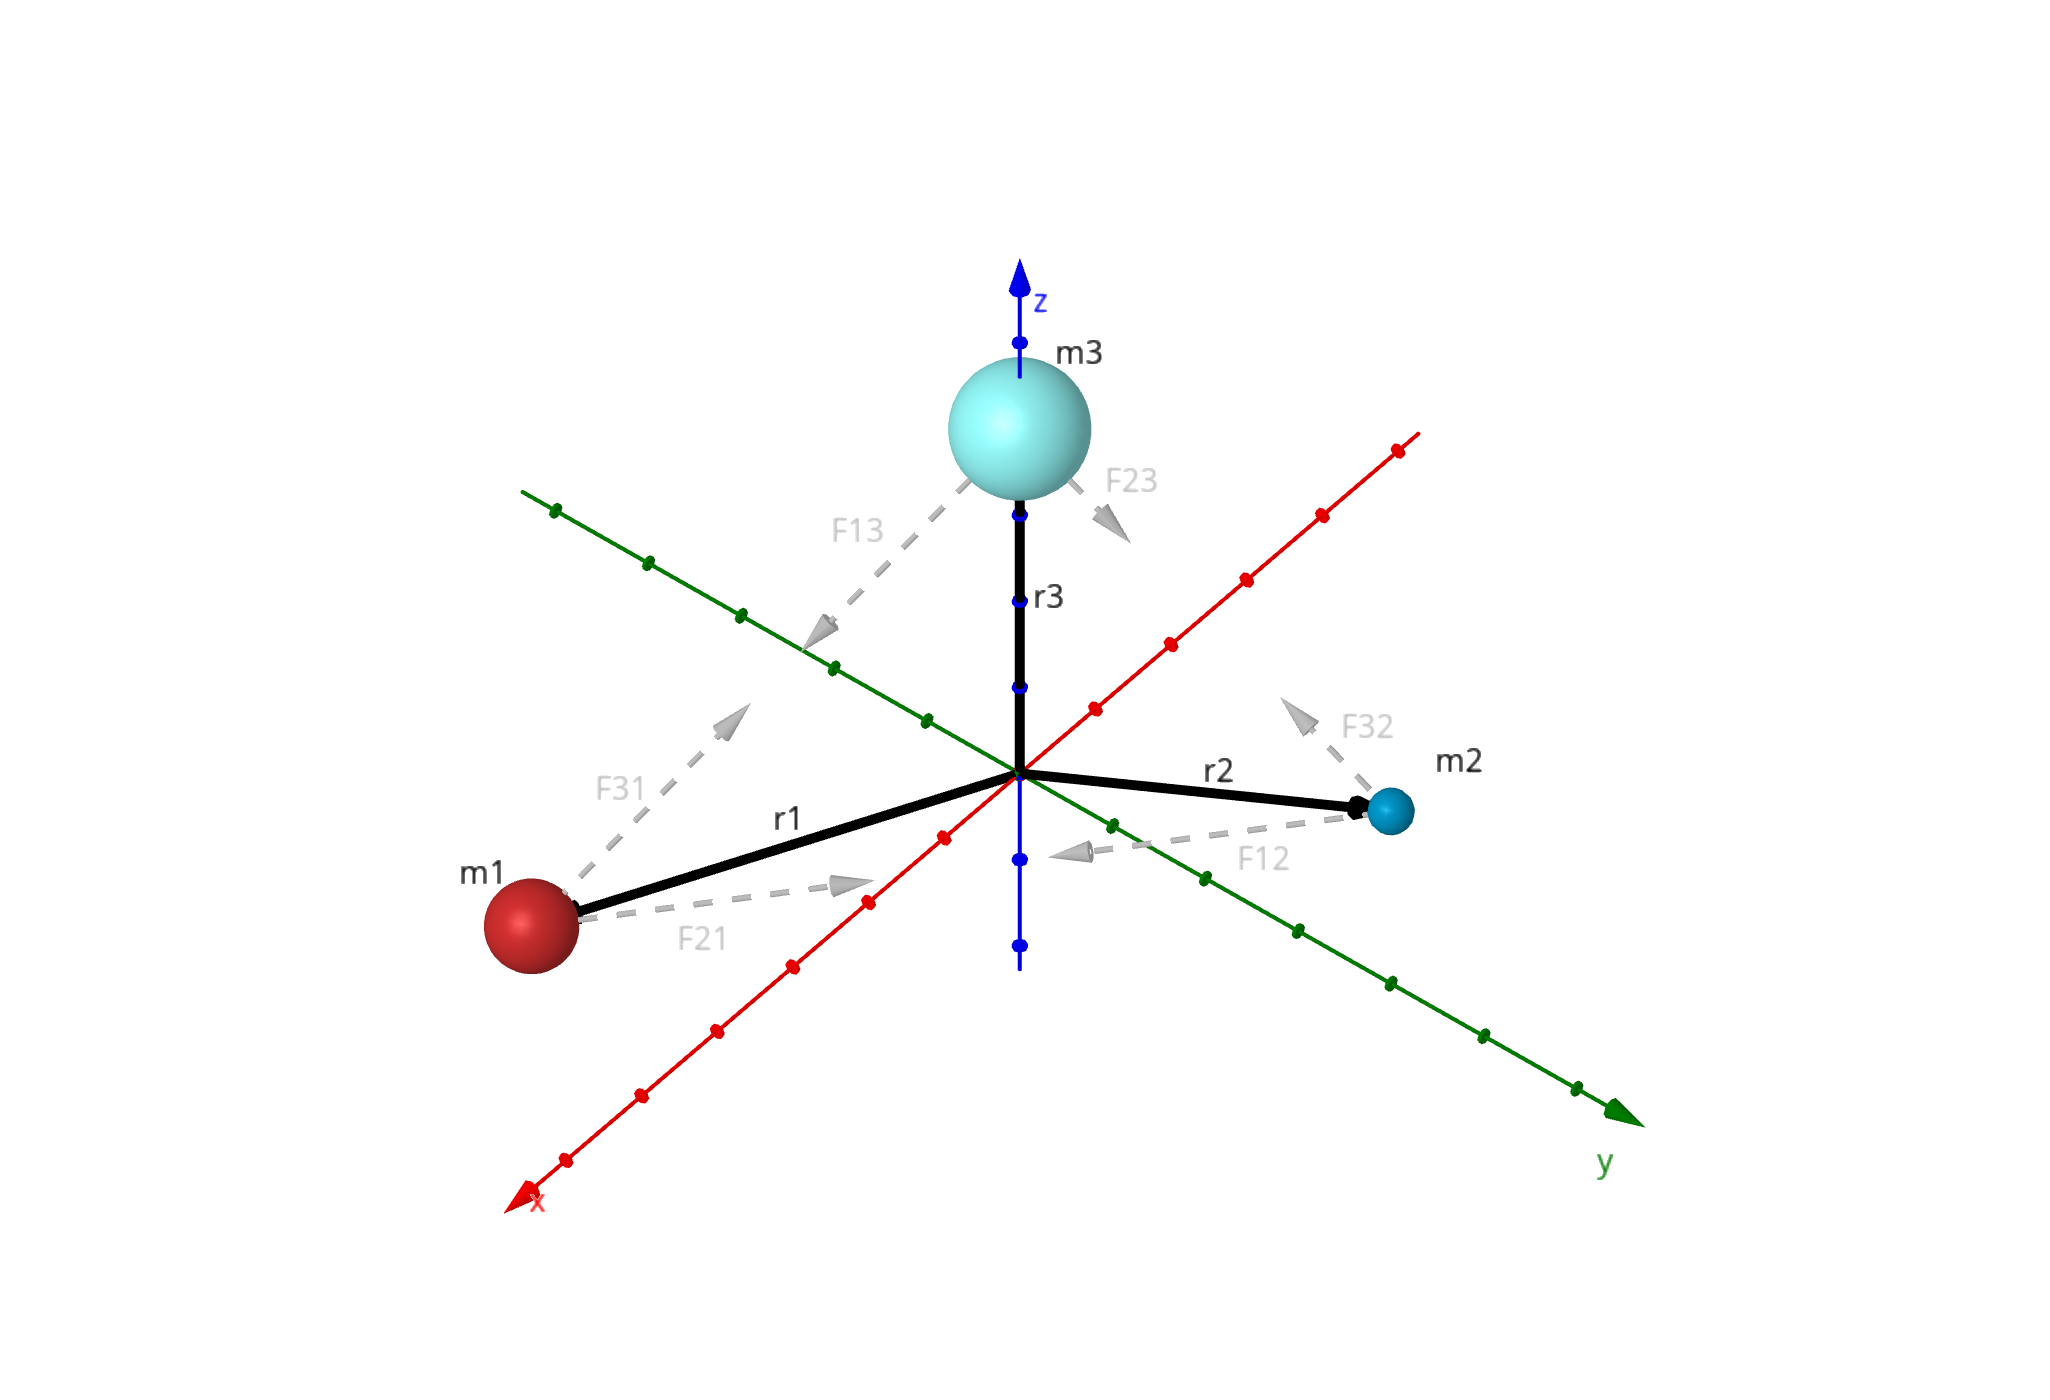
\includegraphics[width=0.9\textwidth]{nbodyexample}
	\caption{<<Схема гравитационного взаимодействия при N=3>>}
	\label{fig:nbodyexample}
\end{figure}
\subsection*{Аналитические решения}
Для случаев $N = 1$ и $N = 2$ существуют точные аналитические решения, при этом для $N = 1$ по законам инерции частица будет двигаться прямолинейно с постоянной скоростью, а в случае $N = 2$ тела будут двигать по одной из кривых второго порядка: эллипсу, гиперболе или параболе.

Для случая $N = 3$ Г.Э. Брунс и А. Пуанкаре показали, что решение общее решение задачи невозможно выразить через алгебраические или через однозначные трансцендентные функции координат и скоростей тел~\cite{markeev}. Однако в 1912 году Зульдман нашёл точное решение задачи, но выраженный в виде бесконечных рядов, использовать которые, однако, невозможно в следствие слишком высокой скорости роста кол-ва вычислений~\cite{markeev}.

Для случаев $N \geq 3$ на текущий момент времени не было найдено точного аналитического решения ни в какой форме, однако существуют решения для отдельных конфигураций~\cite{solution3}.

\subsection*{Метод Эйлера}
Поскольку основная задача данной работы визуализация, а не поиск точного решения задачи n тел, то для решения системы уравнений~\ref{eq:n_system} будут использованы численные методы интегрирования. Одним из таких является метод эйлера, который будет использоваться в данной работе ~\cite{nbody-numeric}~\cite{samarskii}.

Метод эйлера используется для решения задачи Коши вида~\ref{eq:koshi}.
\begin{equation}
	\label{eq:koshi}
	\frac{dy}{dt} = f(t, y(t)), 0 \leq t \leq T, y(0) = y_0
\end{equation}

Пусть на отрезке интегрирования введена сетку $\omega_\tau = {t_i = i\tau, i = 1,2,\dots, n}$, где $\tau = \frac{T}{n}$ -- шаг интегрирования, при этом величина $y_i = y(t_i)$ называется сеточной функцией.
Тогда для этого отрезка используется разностная схема Эйлера~\ref{eq:euler_frac}.
\begin{equation}
	\label{eq:euler_frac}
	\frac{y_{i+1} - y_i}{\tau} = f(t_i, y_i)
\end{equation}

Все значения $y_i$, кроме $y_0$ ищутся итерационно по формуле~\ref{eq:euler_formula}, полученной из~\ref{eq:euler_frac}.

\begin{equation}
	\label{eq:euler_formula}
	y_{i+1} = y_i + \tau f(t_i, y_i)
\end{equation}

Для применения метода эйлера для решения системы уравнений~\ref{eq:n_system} требуется преобразовать её к системе дифференциальных уравнений первого порядка с помощью введения новых переменных - скоростей $v_i$~\ref{n_system_velocities}.

\begin{equation}
	\label{n_system_velocities}
	\begin{cases}
		\frac{d\vec{r_1}}{dt} = \vec{v_1} \\
		\dots \\
		\frac{d\vec{r_N}}{dt} = \vec{v_N} \\
		
		\frac{d\vec{v_1}}{dt} = G\sum_{j=2}^{N}{\frac{m_j}{\vec{r_{j1}}^2}\hat{\vec{r_{j1}}}} \\
		\dots \\
		\frac{d\vec{v_N}}{dt} = G\sum_{j=1, j \neq N}^{N}{\frac{m_j}{\vec{r_{jN}}^2}\hat{\vec{r_{jN}}}} \\
	\end{cases}
\end{equation}

Систему~\ref{n_system_velocities} можно интегрировать методом эйлера используя формулу~\ref{eq:euler_formula}. В результате полученная система~\ref{n_euler_velocities} решает задачу n тел для заданного отрезка интегрирования.

\begin{equation}
	\label{n_euler_velocities}
	\begin{cases}
		\vec{r}_{1}(i+1) = \vec{r}_{1}(i) + \tau \vec{v}_{1}(i) \\
		\dots \\
		\vec{r}_{N}(i+1) = \vec{r}_{N}(i) + \tau \vec{v}_{N}(i) \\
		
		
		\vec{v}_{1}(i+1) = \vec{v}_{1}(i) + \tau G\sum_{j=2}^{N}{\frac{m_j}{\vec{r}_{j1}^2(i)}\hat{\vec{r}}_{j1}(i)} \\
		\dots \\
		\vec{v}_{N}(i+1) = \vec{v}_{N}(i) + \tau G\sum_{j=1, j \neq N}^{N}{\frac{m_j}{\vec{r}_{jN}^2(i)}\hat{\vec{r}}_{jN}(i)} \\
	\end{cases},
\end{equation}
где $\vec{r}_k(i)$ -- радиус-вектор k-ой частицы в i-ый шаг сетки, а $\vec{v}_k(i)$ -- скорость k-ой частицы в i-ый шаг сетки.

\section{Формализованная постановка задачи}

\textbf{Входные данные:}
\begin{itemize}
	\item объекты сцены -- 3-х мерные тела, передающие относительное расположение материальных точек.  Каждый из них представляет собой одно из платоновых тел~\cite{platon-body}. Тело обладает визуальными характеристиками: размер и цвет, и физическими характеристиками материальной точки: масса, положение, линейная скорость;
	\item точечный источник света -- точка создающий свет определённого цвета распространяющийся равномерно во все стороны. Задаётся положением и интенсивностью света;
	\item камера -- сущность которая задаёт плоскость проецирования, видимую область сцены. Задаётся положением, направлениями взгляда и вверх, пирамидой видимости, а также расположением и размерами окна.
\end{itemize}
\textbf{Выходные данные:}
\begin{itemize}
	\item динамически-генерируемая анимация задачи n тел.
\end{itemize}

\begin{figure}[H]
	\centering
	\includesvg[width=0.9\textwidth]{images/ramus/01_A0f}
	\caption{<<Формализованная постановка задачи в нотации idef0>>}
	\label{01_a0f}
\end{figure}

\section{Виды 3-х мерных объектов}
В машинной графике существует 3 основные модели, которыми описываются стереометрические тела~\cite{rodgers}: каркасная, поверхностная и твердотельная модели.

\begin{enumerate}
	\item Каркасная модель -- простейшая из трёх моделей. Объекты в такой модели задаются с помощью множество точек и рёбер, связывающих эти точки.
	\item Поверхностная модель -- модель, задаётся информация о поверхности, ограничивающей объект. Сама поверхность может задаваться аналитически или с помощью полигональной аппроксимации.
	\item Твердотельная модель -- модель, в которой задана поверхность и информация о том, с какой стороны находится материал.
\end{enumerate}

В данной работе не требуется информация о том, с какой стороны расположен материал, однако внутренняя нормаль к поверхности требуется для некоторых алгоритмов, поэтому в данной работе будет использована твердотельная модель.

\section{Способы представления твердотельных моделей}
Существует два подхода к представлению поверхностных моделей в памяти:
\begin{itemize}
	\item \textbf{Аналитический} -- задание поверхностей с помощью описания функций и уравнений. Используются для качественного отображения поверхностей вращения и гладких функций;
	\item \textbf{Полигональная сетка} -- задание поверхности с помощью набора многоугольников. Если с помощью многоугольников нельзя точно задать поверхность, то с помощью них она аппроксимируются.
\end{itemize}

В данной работе в качестве объектов выступают платоновы тела, которые являются многогранниками, так что для них лучше подходит представление в виде полигональной сетки.

\subsection*{Представление полигональных сеток}
Существуют различные способы хранения полигональных сеток в памяти~\cite{colins}.

\subsubsection{Представление точка-точка}
Представление <<точка-точка>> описывает поверхность с помощью списка точек, у каждой из которых хранится список точек, с которыми она соединена. Информация о рёбрах и гранях поверхности не хранятся явно. Представление продемонстрировано на рисунке~\ref{fig:vertex-vertex}.


\begin{figure}[H]
	\centering
	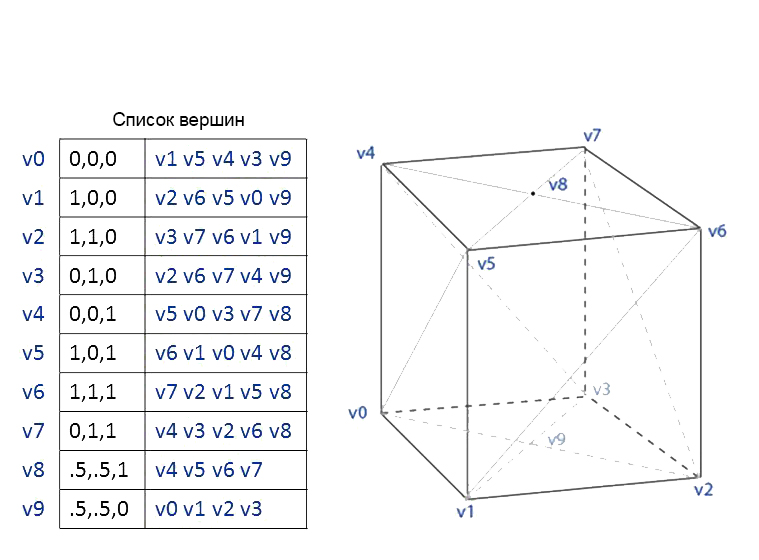
\includegraphics[width=0.7\textwidth]{vertex}
	\caption{<<Представление точка-точка>>}
	\label{fig:vertex-vertex}
\end{figure}


\subsubsection{Представление грань-точка}
Представление <<грань-точка>> описывает поверхность с помощью списка точек и граней. При этом для каждой грани хранятся образующие точки. Представление продемонстрировано на рисунке~\ref{fig:vertex-face}.

\begin{figure}[H]
	\centering
	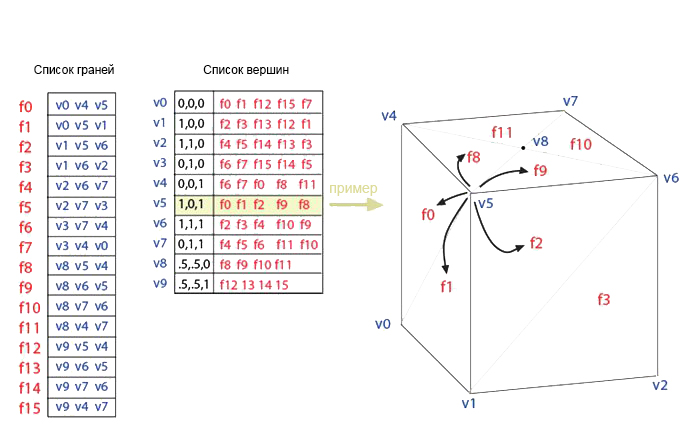
\includegraphics[width=0.7\textwidth]{faces}
	\caption{<<Представление грань-точка>>}
	\label{fig:vertex-face}
\end{figure}

\subsubsection{<<Крылатое>> представление}
При крылатом представлении каждого ребра хранятся две точки, образующие его, две грани, которые он образует и 4 ребра, которые соединены c ним -- по 2 с каждой точкой. Для каждого ребра хранятся ближайшие ребра по часовой и против часовой стрелок.
Представление продемонстрировано на рисунке~\ref{fig:winged}.

\begin{figure}[H]
	\centering
	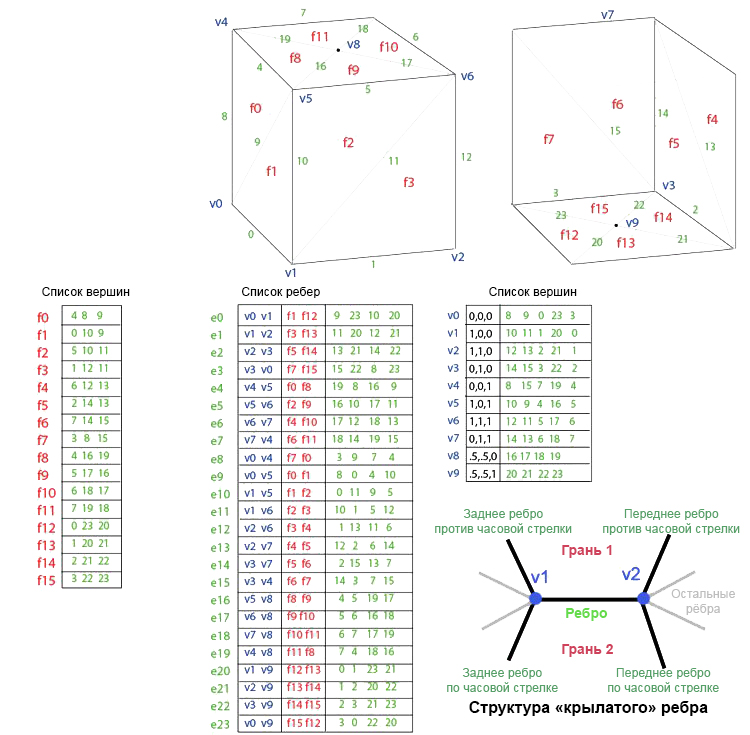
\includegraphics[width=0.7\textwidth]{winged}
	\caption{<<Крылатое представление>>}
	\label{fig:winged}
\end{figure}

В таблице~\ref{tbl:mesh-structs} представлено сравнение способов хранения полигональных сеток.

\begin{longtable}{|p{0.2\textwidth}|p{0.25\textwidth}|p{0.25\textwidth}|p{0.2\textwidth}|}
	\caption{Сравнение представлений полигональных сеток} \label{tbl:mesh-structs} 
	\\
	\hline
	\textbf{Критерий} & \textbf{<<Точка-точка>>} & \textbf{<<Грань-точка>>} & \textbf{<<Крылатое>>} \\
	\hline
	\endfirsthead
	\caption{Сравнение представлений полигональных сеток}
	\\
	\hline
	\textbf{Критерий} & \textbf{<<Точка-точка>>} & \textbf{<<Грань-точка>>} & \textbf{<<Крылатое>>} \\
	\hline
	\endhead
	\hline
	\endfoot
	\endlastfoot
	Кол-во указателей для хранения куба\cite{colins} & 24 & \textbf{30} & 192 \\
	\hline
	Получение всех граней & неявное & \textbf{явное} & явное \\
	\hline
	Получение всех рёбер & неявное & \textbf{неявное} & явное \\
	\hline
\end{longtable}

В данной работе было выбрано представление <<грань-точка>>, так как оно позволяет получать список граней без дополнительных операций, а также не требует для хранения дополнительной информации.

\section{Алгоритмы удаления невидимых поверхностей}

Алгоритм удаления невидимых поверхностей является наиболее вычислительно сложной задачей в компьютерной графике~\cite{rodgers}. На данном этапе определяются объекты или их части, которые буду отрисованы на экране.

Одна из классификаций алгоритмов -- по системе координат, в которой они работают:
\begin{itemize}
	\item\textbf{В пространстве объектов} -- имеют дело с физической системой координат, в которой заданы объекты. Точность ограничена точностью вычислений.
	\item\textbf{В пространстве экрана} -- имеют дела с системой координат, связанной с экраном. Точность ограничена разрешением экрана.
\end{itemize}

При выборе алгоритма удаления невидимых поверхностей, важно учесть, что изображение будет строиться динамически в реальном времени и, что объекты будут иметь небольшой размер и отдалены от камеры, так как они созданы для визуализации положения материальной точки, размеры которой малы.

Будут рассмотрены 4 алгоритма удаления невидимых поверхностей~\cite{ngtu}:

\begin{enumerate}
	\item алгоритм Робертса;
	\item алгоритм обратной трассировки лучей;
	\item алгоритм Варнока;
	\item алгоритм использующий z-буфер.
\end{enumerate}

\subsection*{Алгоритмы в объектном пространстве}
\subsubsection{Алгоритм Робертса}
Алгоритм Робертса -- первое известное решение задачи удаления невидимых поверхностей~\cite{rodgers}. Для работы алгоритма требуются выпуклые тела. Алгоритм состоит из 4-х этапов.

\textbf{Первый этап} -- подготовка матрицы тела. Матрица тела -- матрица, хранящая информацию об уравнениях, задающих плоскости всех граней. Имеет размерность $4*n$, где n -- число граней тела.

\begin{equation}
	\label{eq:body_matrix}
	V = \begin{pmatrix}
		a_1\ a_2\ \dots\ a_n \\
		b_1\ b_2\ \dots\ b_n \\
		c_1\ c_2\ \dots\ c_n \\
		d_1\ d_2\ \dots\ d_n 
	\end{pmatrix},
\end{equation}
где $ a_ix + b_iy + c_iz + d_i = 0 $ -- уравнение i-ой грани. Матрица должна быть сформирована так, чтобы при умножению на неё точку внутри тела получался вектор положительных чисел.

\textbf{Второй этап} -- удаление нелицевых граней. На данном этапе удаляются грани, которые экранируются самими объектами.

\textbf{Третий этап} -- удаление рёбер, экранируемых другими телами. Для этого для каждого оставшегося ребра нужно пустить луч из точки взгляда к точке ребра. Если луч проходит через другие грани, значит эта точка отрезка экранируется. 

\textbf{Четвёртый этап} -- создание рёбер соединения граней. Для этого запоминаются все точки протыкания в предыдущем пункте и попарно соединяются отрезками. Далее эти отрезки также проверяются на экранирование, как и в 3-ем пункте.

Алгоритм обеспечивает высокую точность вычислений, но сложный вычислительно и налагает условие выпуклости на тела.

\subsubsection{Алгоритм обратной трассировки лучей}
В данном алгоритме удаление невидимых граней происходит за счёт построения луча из точки обзора через каждый пиксель экрана~\cite{gabriella}. Таким образом на экран попадают лишь объекты, пересечение которых с лучом происходит ближе к точке обзора. Трассировку луча можно продолжить отражением и преломления по законам оптики для моделирования зеркального отражения.

\subsection*{Алгоритмы в пространстве экрана}
\subsubsection{Алгоритм Варнока}

Алгоритм Варнока основан на идее, что для обработки областей с малой плотностью информации мозг человека тратит малое количество времени, а с большой плотностью — больше.

Идея алгоритма в том, чтобы разбивать экран на окна и подокна до тех пор, пока его содержимое не будет элементарным для визуализации, или пока не будет достигнут предел разрешения. На рисунке~\ref{fig:varnok} представлен пример разбиения экрана алгоритмом Варнока.

\begin{figure}[H]
	\centering
	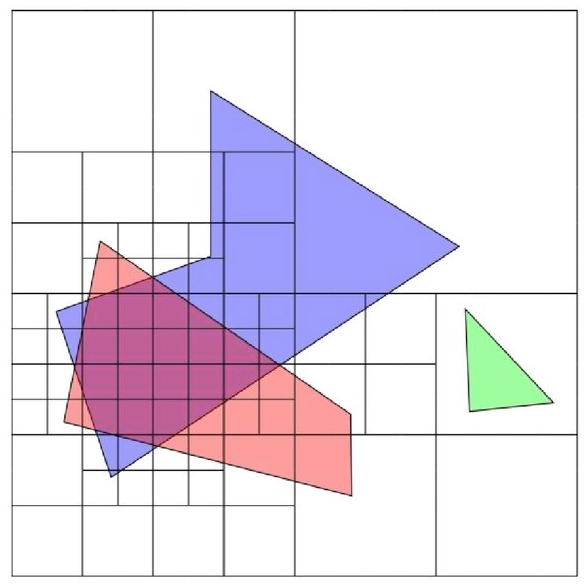
\includegraphics[width=0.4\textwidth]{varnok}
	\caption{<<Пример работы алгоритма Варнока>>}
	\label{fig:varnok}
\end{figure}

\subsubsection{Алгоритм использующий z-буфер}
Алгоритм z-буфера — один из широко используемых алгоритмов отрисовки удаления невидимых поверхностей.

Основой алгоритма является два буфера, которые имеют размеры экрана в пикселях:

\begin{itemize}
	\item \textbf{Буфер кадра} — используется для хранения значения интенсивности(цвета) каждого пикселя, который будет отрисован на экране. По сути хранит в себе то, как экран будет выглядеть в следующем кадре.
	\item \textbf{Буфер глубины(z-буфер)} — Используется для хранения глубины каждого пикселя, описанного в буфере кадра. Нужен для определения видимых граней.
\end{itemize}

Предварительно алгоритм требует проецирование объекта в пространство экрана. Алгоритм растеризует объект и сохраняет его в буфере кадра и глубины, при этом, если глубина очередного пикселя больше, чем уже сохранённого в буфере, то этот пиксель пропускается.

Но при этом алгоритм требует большего объёма памяти, для хранения буферов~\cite{rodgers}, чем другие алгоритмы, но он обрабатывает только те пиксели, в которых есть объекты.

\subsection*{Выбор алгоритма удаления невидимых поверхностей}

В таблице~\ref{tbl:invisible} представлено сравнение методов удаления невидимых поверхностей.

\begin{longtable}{|p{0.2\textwidth}|p{0.23\textwidth}|p{0.14\textwidth}|p{0.14\textwidth}|p{0.16\textwidth}|}
	\caption{Сравнение алгоритмов удаления невидимых поверхностей} \label{tbl:invisible} 
	\\
	\hline
	\textbf{Критерий} & \textbf{Трассировка лучей} & \textbf{Робертс} & \textbf{Варнок} & \textbf{Z-буфер} \\
	\hline
	\endfirsthead
	\caption{Сравнение алгоритмов удаления невидимых поверхностей}
	\\
	\hline
	\textbf{Критерий} & \textbf{Трассировка лучей} & \textbf{Робертс} & \textbf{Варнок} & \textbf{Z-буфер} \\
	\hline
	\endhead
	\hline
	\endfoot
	\endlastfoot
	Обрабатываются ли пустые пиксели? & Да & Нет & Да & \textbf{Нет} \\
	\hline
	Дополнительная память & Нет & Нет & Да, 1 буфер размером с количество пикселей & \textbf{Да, 2 буфера размером с количество пикселей} \\
	\hline
	Требует информацию о рёбрах тела & Нет & Да & Нет & \textbf{Нет} \\
	\hline
	Вычислительная сложность & $O(n_{\text{объекты}}*n_{\text{пиксели}} * n_{\text{лучи}})$ & $O(n_{\text{объекты}}^2)$ & $O(n_{\text{объекты}}*n_{\text{подокна}})$ & \textbf{$O(n_{\text{объекты}}*n_{\text{пиксели проекции}})$} \\
	\hline
\end{longtable}

Для данной работы оптимальным является алгоритм z-буфера, так как он является достаточно производительным для динамических сцен, не обрабатывает пустые пиксели, которых будет больше непустых, так как объекты небольшие, а дополнительные затраты памяти не являются критическими.

\section{Модель освещения}
Модели освещения в компьютерной графике делятся на 2 больших класса: глобальные и локальные.

Глобальные модели освещения учитывают отражённый и преломлённый свет от других объектов, однако расчёт такой модели требует трассировку лучей, поэтому не могут быть реализованы в этой работе.

Локальные модели освещения учитывают только прямой свет от источника до рассматриваемого объекта. В данной работе будет использована модель Ламберта~\cite{kazancev}, для расчёта освещения.

Отражённый свет зависит от характеристик и положения источника, относительно тела. При этом свет может быть отражён диффузно и зеркально. Зеркальное отражение не учитывается в модели ламберта. Диффузное отражённый свет испускается во все стороны равномерно. Интенсивность отражаемого диффузного света зависит закону Ламберта~\cite{kazancev}:
\begin{equation}
	\label{eq:lambert1}
	I = I_{l}k_dcos(\phi),\ 0\leq\phi\leq\frac{\pi}{2},
\end{equation}
где
\begin{itemize}
	\item $I$ -- интенсивность отражённого света;
	\item $I_s$ -- интенсивность источника света
	\item $k_d$ -- коэффициент диффузного отражения тела
	\item $\phi$ -- угол между нормалью к поверхности в точке падения и направлением света.
\end{itemize} 

Свет, отражённый от других объектов в локальных моделях заменяется на рассеянный свет:
\begin{equation}
	\label{eq:lambert2}
	I = I_ak_a + I_{l}k_dcos(\phi),\ 0\leq\phi\leq\frac{\pi}{2},
\end{equation}
где $I_a$ -- интенсивность рассеянного света, а $k_a$ -- коэффициент диффузного отражения рассеянного света. 

\section{Метод учёта теней}

Тени делят на проекционные и собственные. Собственные тени образуются телами на себя, проекционные -- образованные другими телами.

Для учёта проекционных теней, будет использован метод теневых карт~\cite{gabriella}. Данный метод является модификацией z-буфера.

\begin{enumerate}
	\item Для каждого источника света:
	\begin{enumerate}
		\item преобразовать объекты в пространство источника света;
		\item построить буфер глубины методом z-буфера;
	\end{enumerate}
	
	\item Для каждой точки из буфера кадра:
	\begin{enumerate}
		\item преобразовать точку в пространство источника света;
		\item если глубина точки больше глубины соответствующего значения буфера глубины:
		\item точка в тени;
		\item иначе:
		\item точка освещена. 
	\end{enumerate}
\end{enumerate}

Так как в работе будут использоваться точечные источники света, то для каждого источника необходимо будет построить 6 теневых карт, которые образуют куб, описывающий источник.

Полученные тени будут выглядеть ступенчато (рисунок~\ref{fig:shadowstep}), так как их точность ограничена разрешением теневого буфера. Для точного учёта собственных теней будет использован метод, основанный на первых 2-х этапах алгоритма Робертса: если грань относительно источника света является нелицевой, то она находится в тени относительно этого источника света~\cite{rodgers}.

\begin{figure}[H]
	\centering
	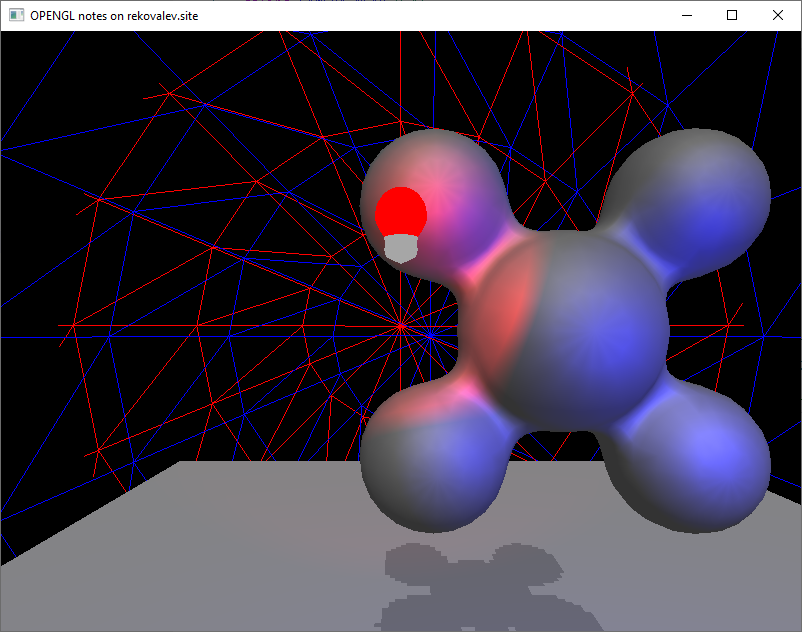
\includegraphics[width=0.8\textwidth]{shadowstep}
	\caption{<<Пример ступенчатости теней, созданных теневыми картами~\cite{shadowstep}>>}
	\label{fig:shadowstep}
\end{figure}


\section*{Вывод}

В результате аналитической части была описана математическая модель рассматриваемой задачи, а также описан метод её решения. Были рассмотрены теоретические сведения о способах представления объектов программно и методы преобразования этих объектов для отображения на экране. Также были выбраны методы и алгоритмы, которые будут использоваться в данной работе.

\clearpage
